\icode{E-MI-SU-L3-261105-001}
（多选）
如图所示，上表面光滑的斜面静置于粗糙水平面上，斜面质量\(M=\)\,\qty{3.2}{kg}，倾角\(\theta =\)\,\qty{37}{\degree}，外面顶端固定有光滑轻质滑轮，质量\(m =\)\,\qty{1}{kg}的物块系于轻绳一端，轻绳另一端跨过滑轮系于地而上，斜面左侧的轻绳保持竖直，斜面上方的轻绳与斜面平行。已知重力加速度大小\(g =\)\,\qty{10}{m/s^2}，\(\sin\)\qty{37}{\degree}=0.6，\(\cos\)\qty{37}{\degree}=0.8，最大静摩擦力等于滑动摩擦力。下列说法正确的是\paren[]

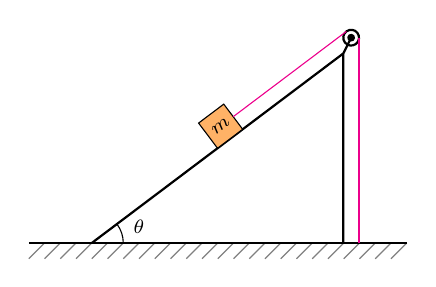
\begin{tikzpicture}[font=\scriptsize]
	\begin{scope}[rotate=37]
		\coordinate (P) at(4.28,.04);
		\draw[thick] (0,0)--(4,0)--++(-127:2.4) (4,0)--(4.2,.1) (4.2,.1) circle(.1);
		\fill (4.2,.1) circle(.05);
		\draw[fill=orange!60] (2,0) rectangle(2.4,.4)node[midway,rotate=37]{\(m\)};
		\draw[magenta] (2.4,.2)--(4.2,.2);
	\end{scope}
	\foreach \x in {-.8,-.6,...,3.8}
		\draw[gray] (\x,-.2)--++(.2,.2);
	\draw[thick] (-.8,0)--(4,0);
	\draw (.4,0) arc(0:37:.4);
	\draw[magenta] (P)--(P|-3,0);
	\node at(.6,.2){\(\theta\)};
\end{tikzpicture}
\begin{choices}
	\item 轻绳的拉力大小为\qty{8}{N}
	\item 水平面对斜而的弹力大小为\qty{48}{N}
	\item 水平面对斜而的摩擦力大小为\qty{4.8}{N}
	\item 剪断轻绳瞬间，为使斜面保持静止，斜面与水平面间的动摩擦因数至少为0.125
\end{choices}	
\begin{answer}
	BD\qquad 提示：将物块、斜面与定滑轮、轻绳看作一个整体
\end{answer}